\chapter{Despliegue de atención} \label{appendixB}
En el caso en el que trabajamos con un modelo formado por bloques dispuestos secuencialmente con un único cabezal de atención, podemos aproximar el comportamiento global de la atención como el producto de las matrices de pesos de atención de los sucesivos bloques. Esta técnica, relativamente novedosa, recibe el nombre de despliegue de atención (\textit{attention rollout}).

\begin{definition}{Despliegue de atención (\textit{attention rollout}) \cite{abnar2020quantifying}}
  Sea \( (\mathbb{V}^*, \mathbb{P}) \) un lenguaje, \( x \in \mathbb{V}^* \) una secuencia y \( \texttt{GPT}(\smallbullet \mid \theta) \) la función definida en el \cref{algo:gpt} con un único cabezal de atención y \( L_\text{dec} \) bloques codificador.

  Consideremos la sucesión \( \Set{W_i}_{i = 1}^{L_\text{dec}} \) de \textit{matrices de pesos de atención} asociada a evaluar \( \texttt{GPT}(x \mid \theta) \). Llamamos despliegue de atención al término \( A_{L_\text{dec}} \) de la sucesión \( \Set{A_i} \) tal que:
  \begin{align}
    A_{i} = (W_i + I)A_{i - 1}  & \text{ para \( i = 2, …, L_\text{dec} \)} \\
    A_1 = W_1
  \end{align}
\end{definition}

En el caso habitual, en el que hay presentes varios cabezales de atención la evaluación de GPT sobre una secuencia \( x \) genera una sucesión de \textit{matrices de pesos} de la forma \( \Set{W_{ij}}_{i = 1, j = 1}^{L_\text{dec}, H} \) y la forma habitual de implementar el despliegue de atención es calcularlo sobre la matriz de pesos de atención promedio
\begin{equation} \label{eq:attention_weight}
    \widetilde{W}_i = \frac{1}{H} \sum_j W_{ij}
\end{equation}
o calculando el mínimo (o el máximo), esto es:
\begin{equation} \label{eq:attention_min}
    \widetilde{W}_i = \min_j  W_{ij}
\end{equation}

Otra posibilidad es calcularlo sobre un único cabezal, es decir calcular el despliegue de atención sobre la sucesión \( W_{ij_0} \) para un determinado \( j_0 \). La \cref{fig:attention_rollout} muestra el resultado de aplicar estas técnicas sobre una misma secuencia en el modelo GPT-2 entrenado. 

Aunque estas técnicas solo ofrecen una aproximación, que en el caso de modelos con un número significativo de cabezales y bloques puede ser muy imprecisa, del funcionamiento del modelo son una herramienta muy valiosa para profundizar en el funcionamiento de los \textit{transformer}. 

\begin{figure}[tb]
    \centering
    \begin{subfigure}[b]{0.49\textwidth}
        \centering
        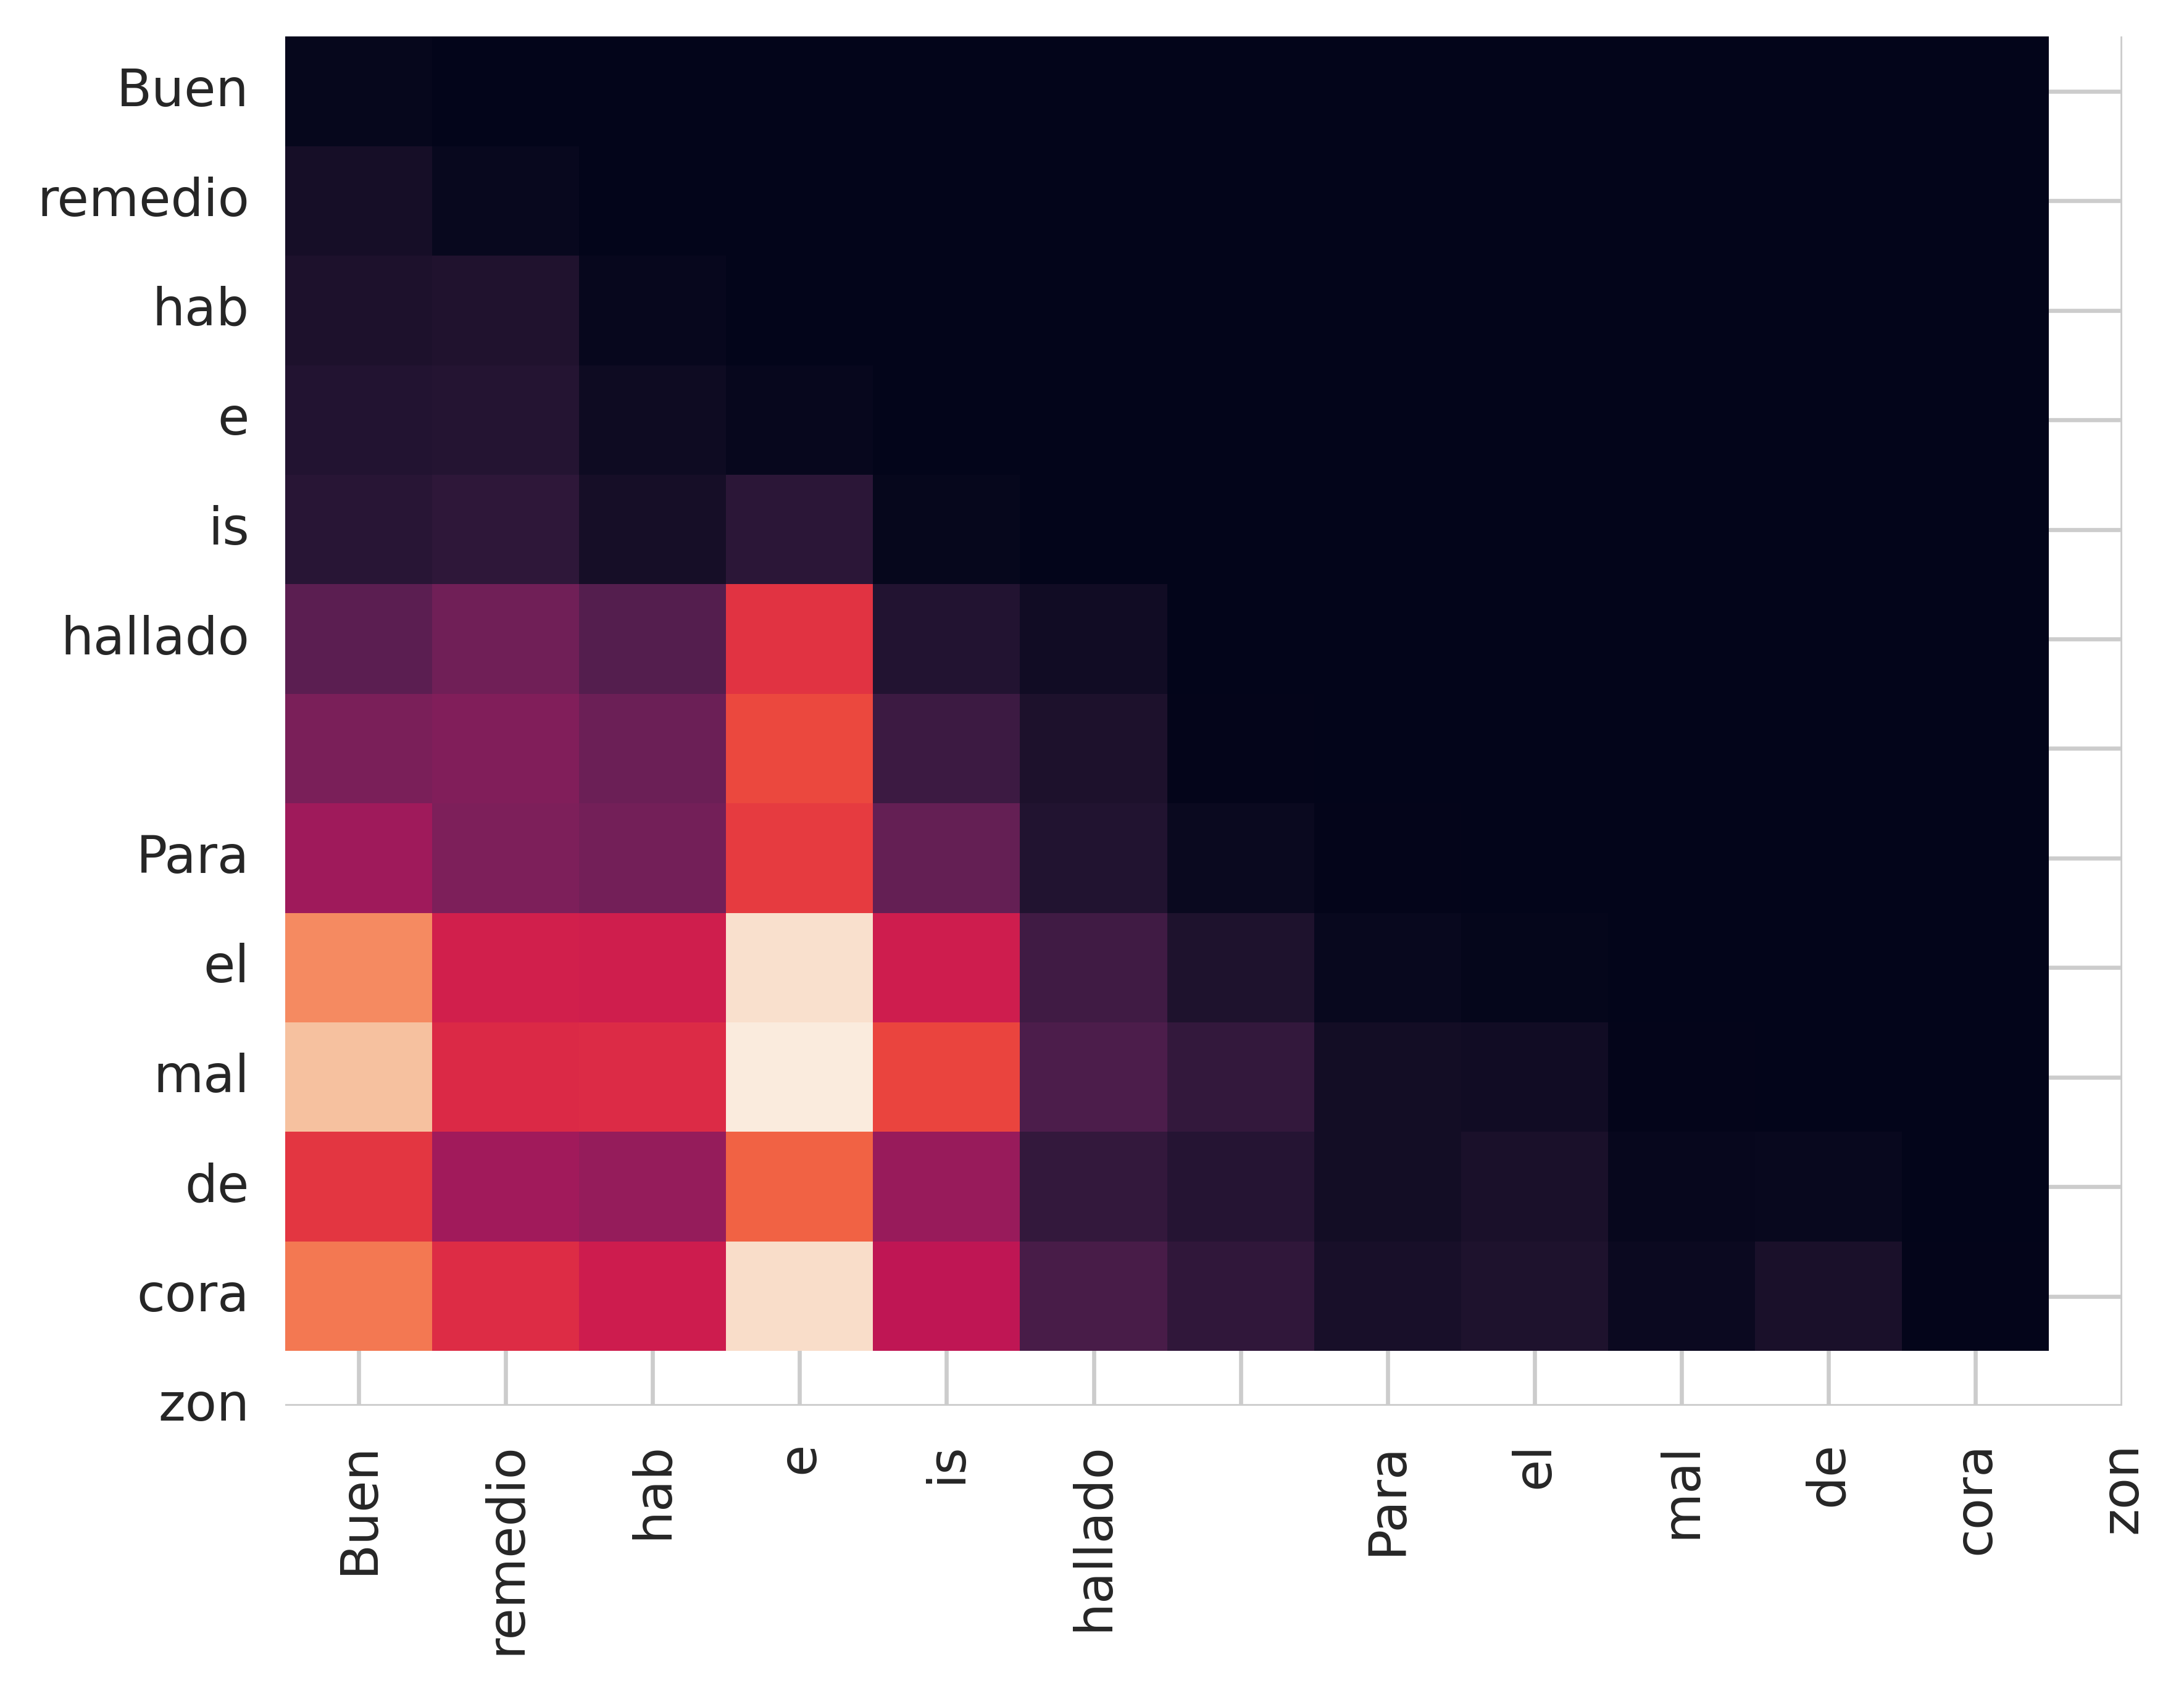
\includegraphics[width=\textwidth]{figures/chapter5/rollout_4.png}
        \caption{Despligue de atención para un cabezal de atención concreto}
    \end{subfigure}
    \smallskip
    \begin{subfigure}[b]{0.49\textwidth}
        \centering
        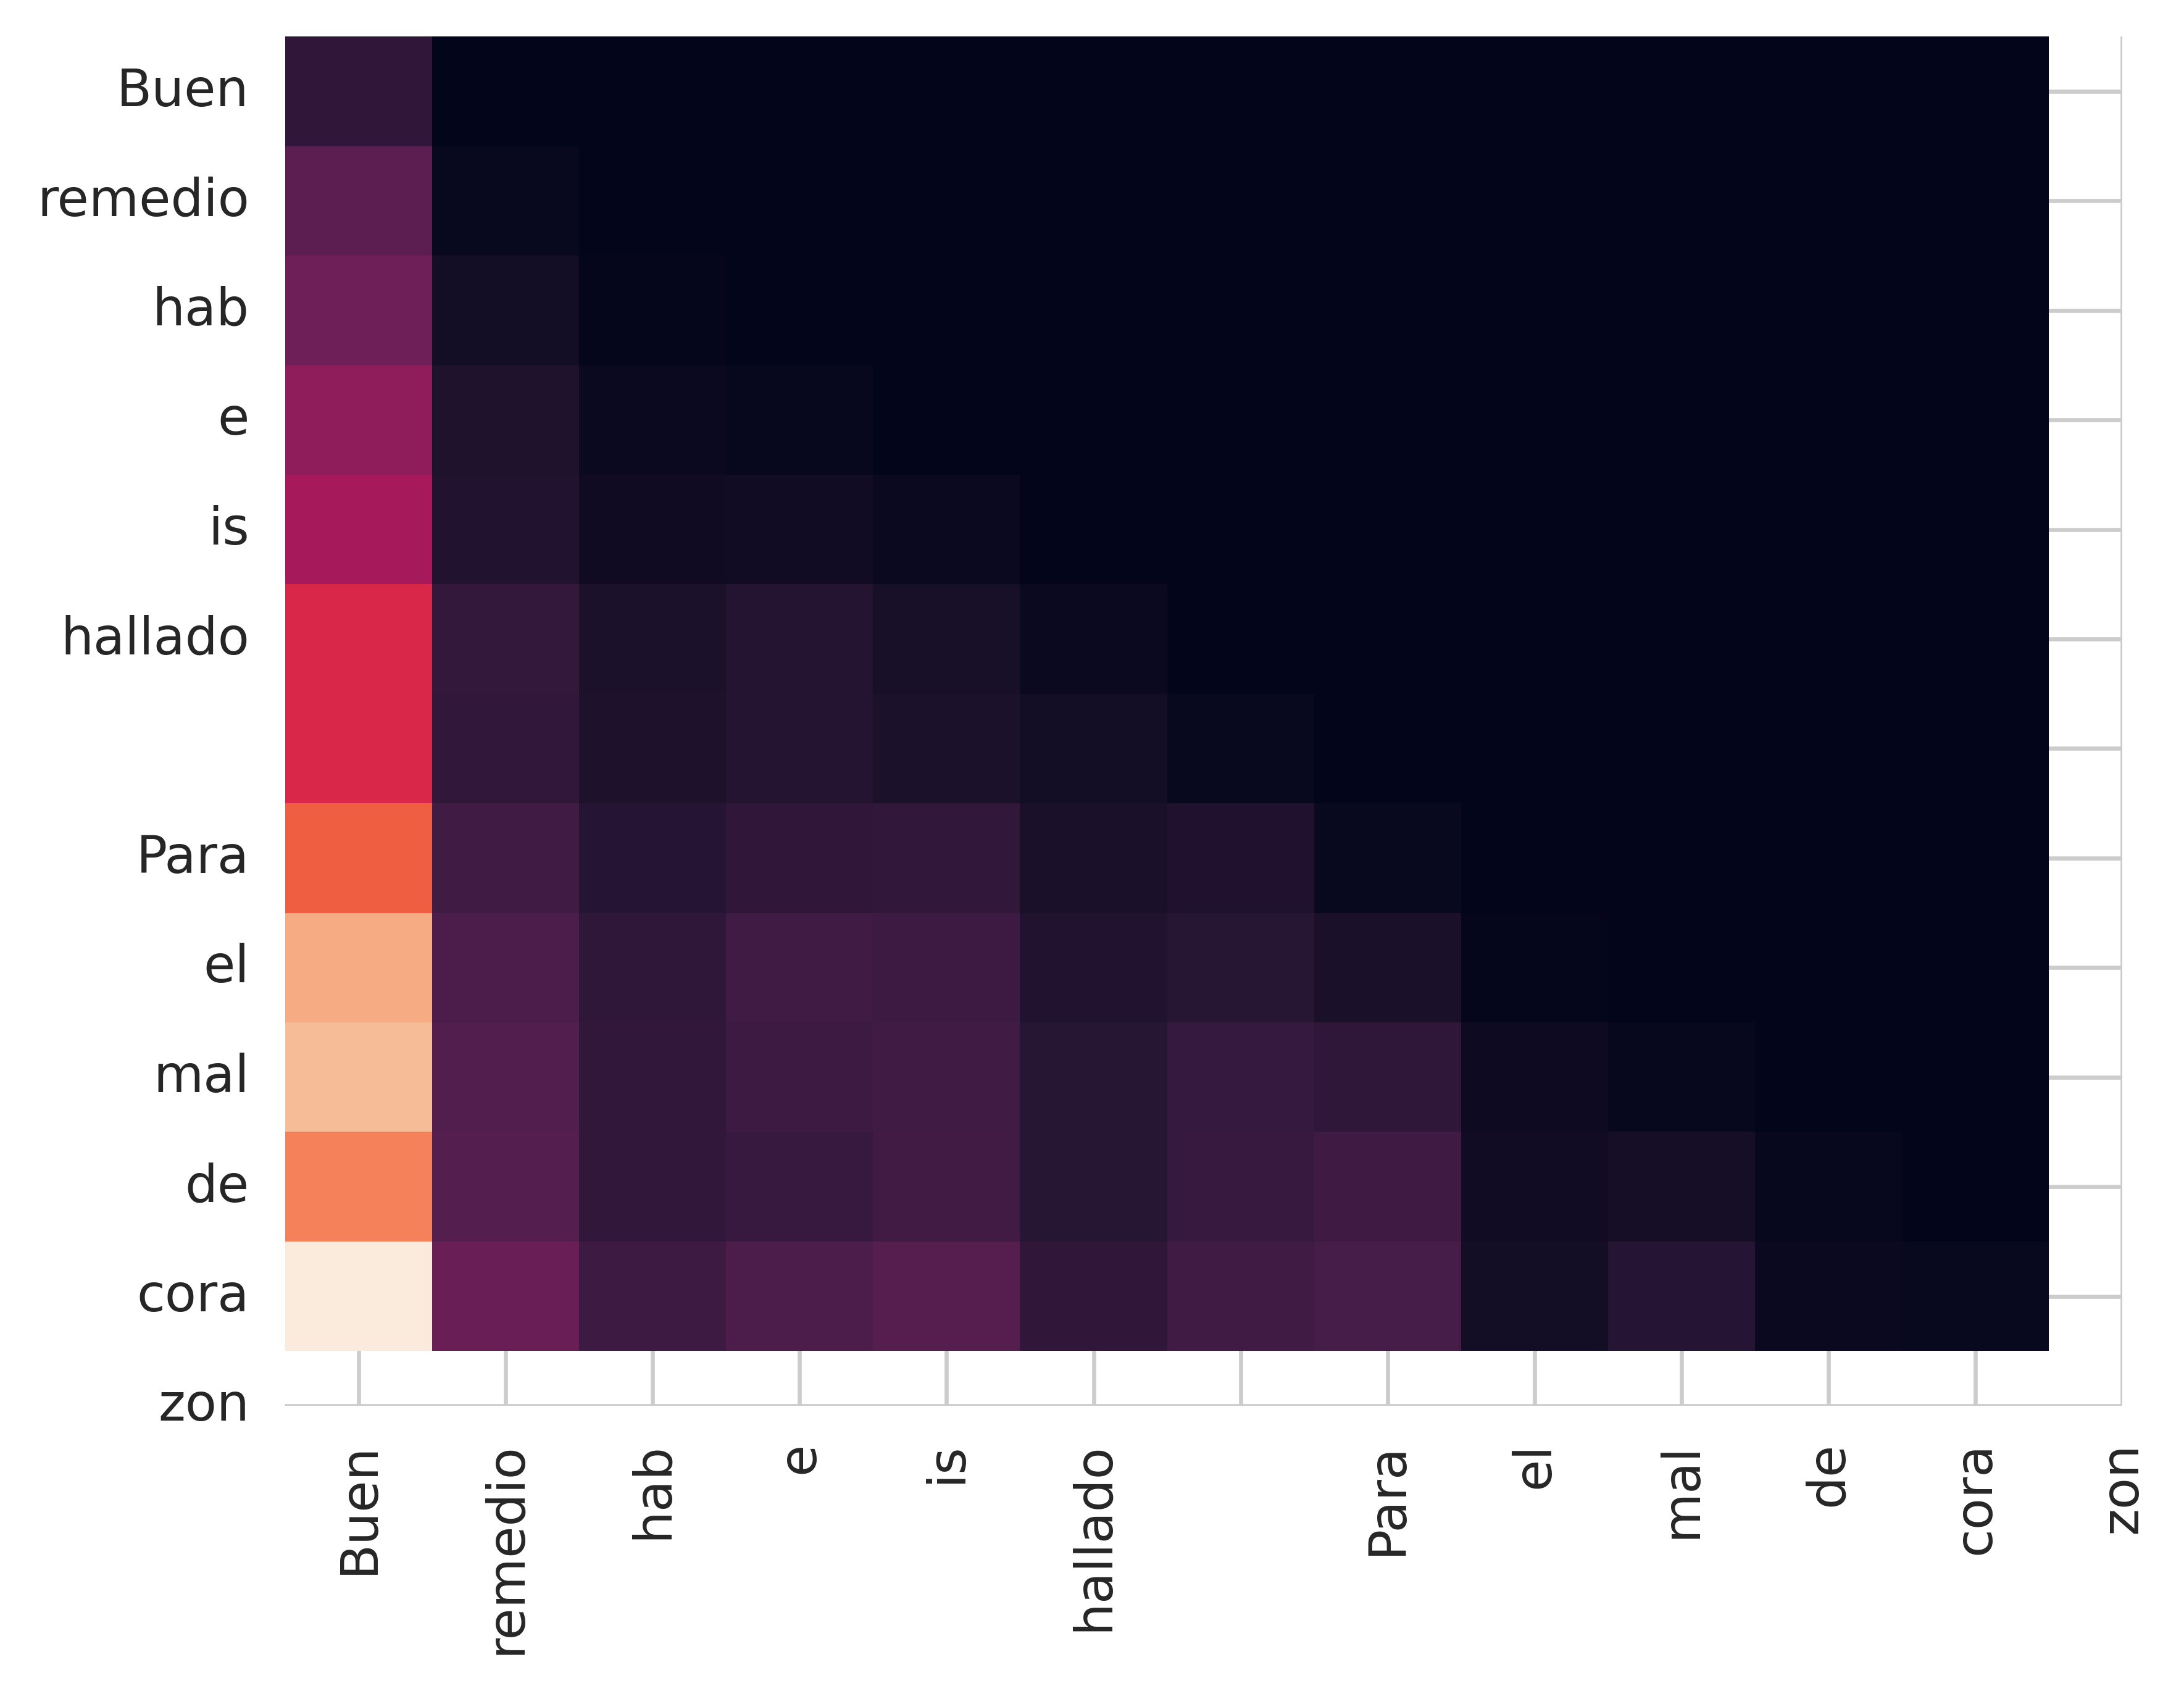
\includegraphics[width=\textwidth]{figures/chapter5/rollout_avg.png}
        \caption{Despliegue de atención sobre la matriz de pesos de atención promedio (\cref{eq:attention_weight})}
    \end{subfigure}
    \bigskip
    \begin{subfigure}[b]{0.49\textwidth}
        \centering
        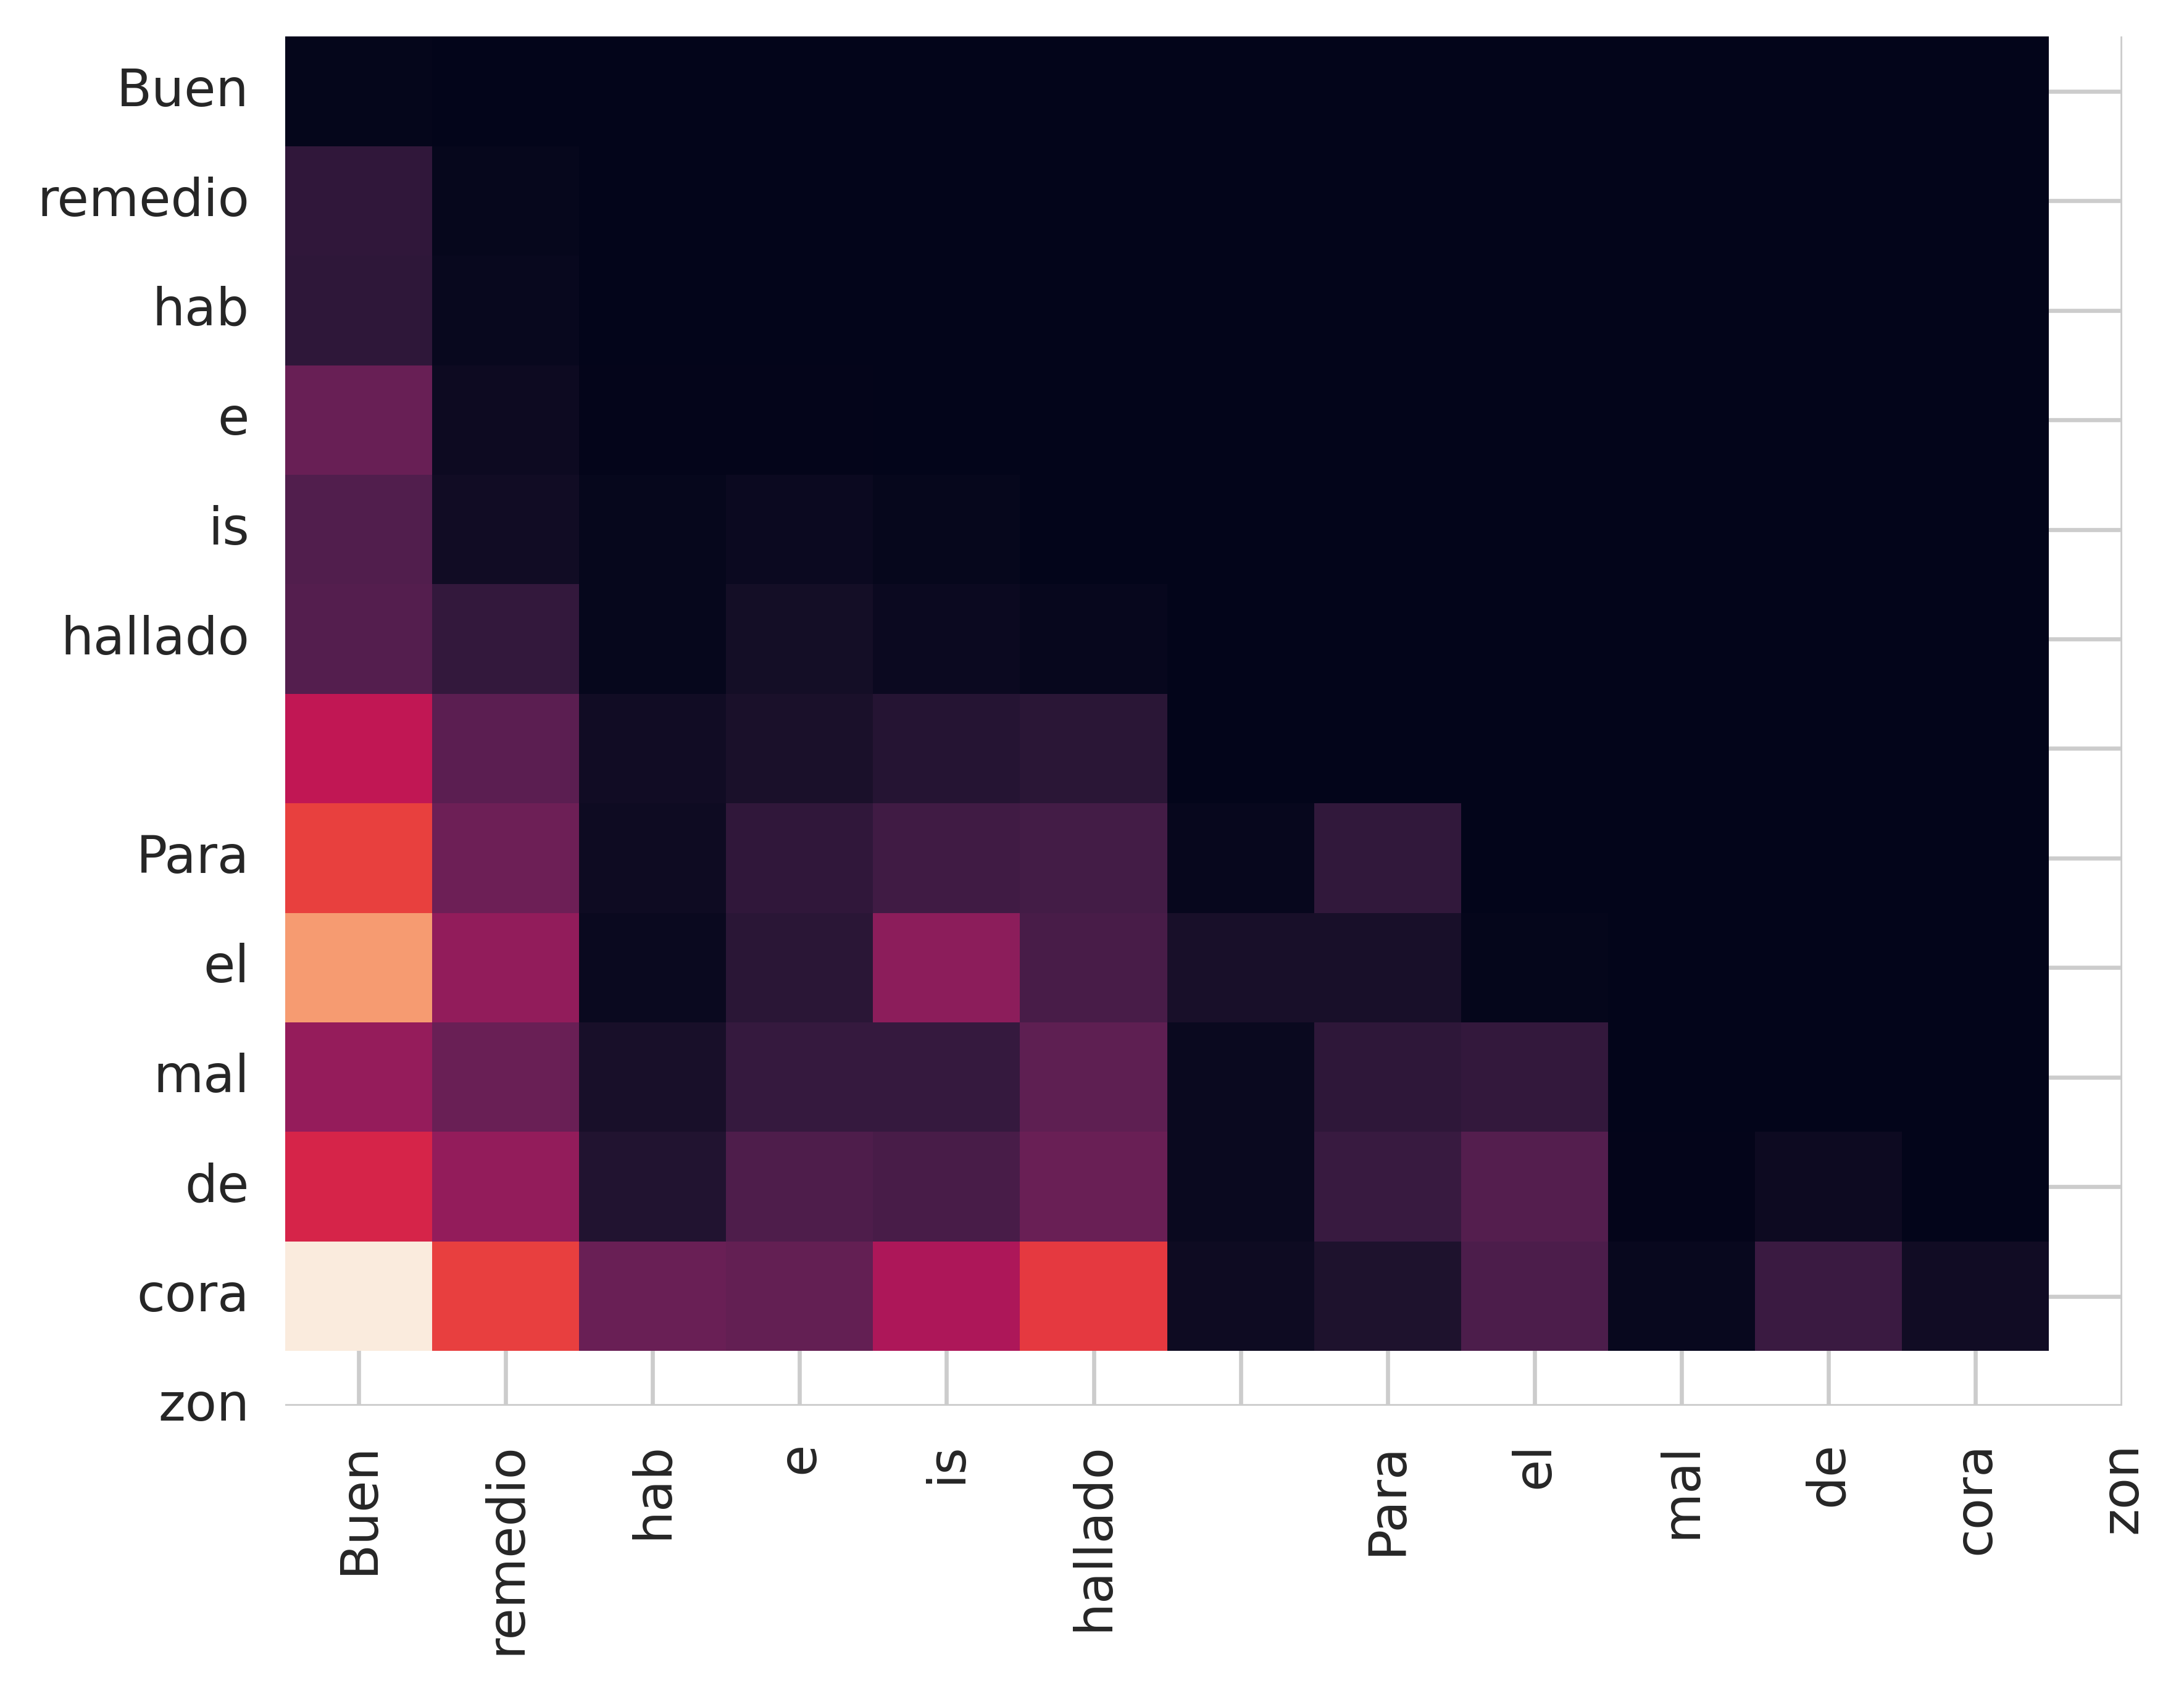
\includegraphics[width=\textwidth]{figures/chapter5/rollout_min.png}
        \caption{Despligue de atención sobre la matriz de pesos de atención mínima (\cref{eq:attention_min})}
    \end{subfigure}
    \smallskip
    \begin{subfigure}[b]{0.49\textwidth}
        \centering
        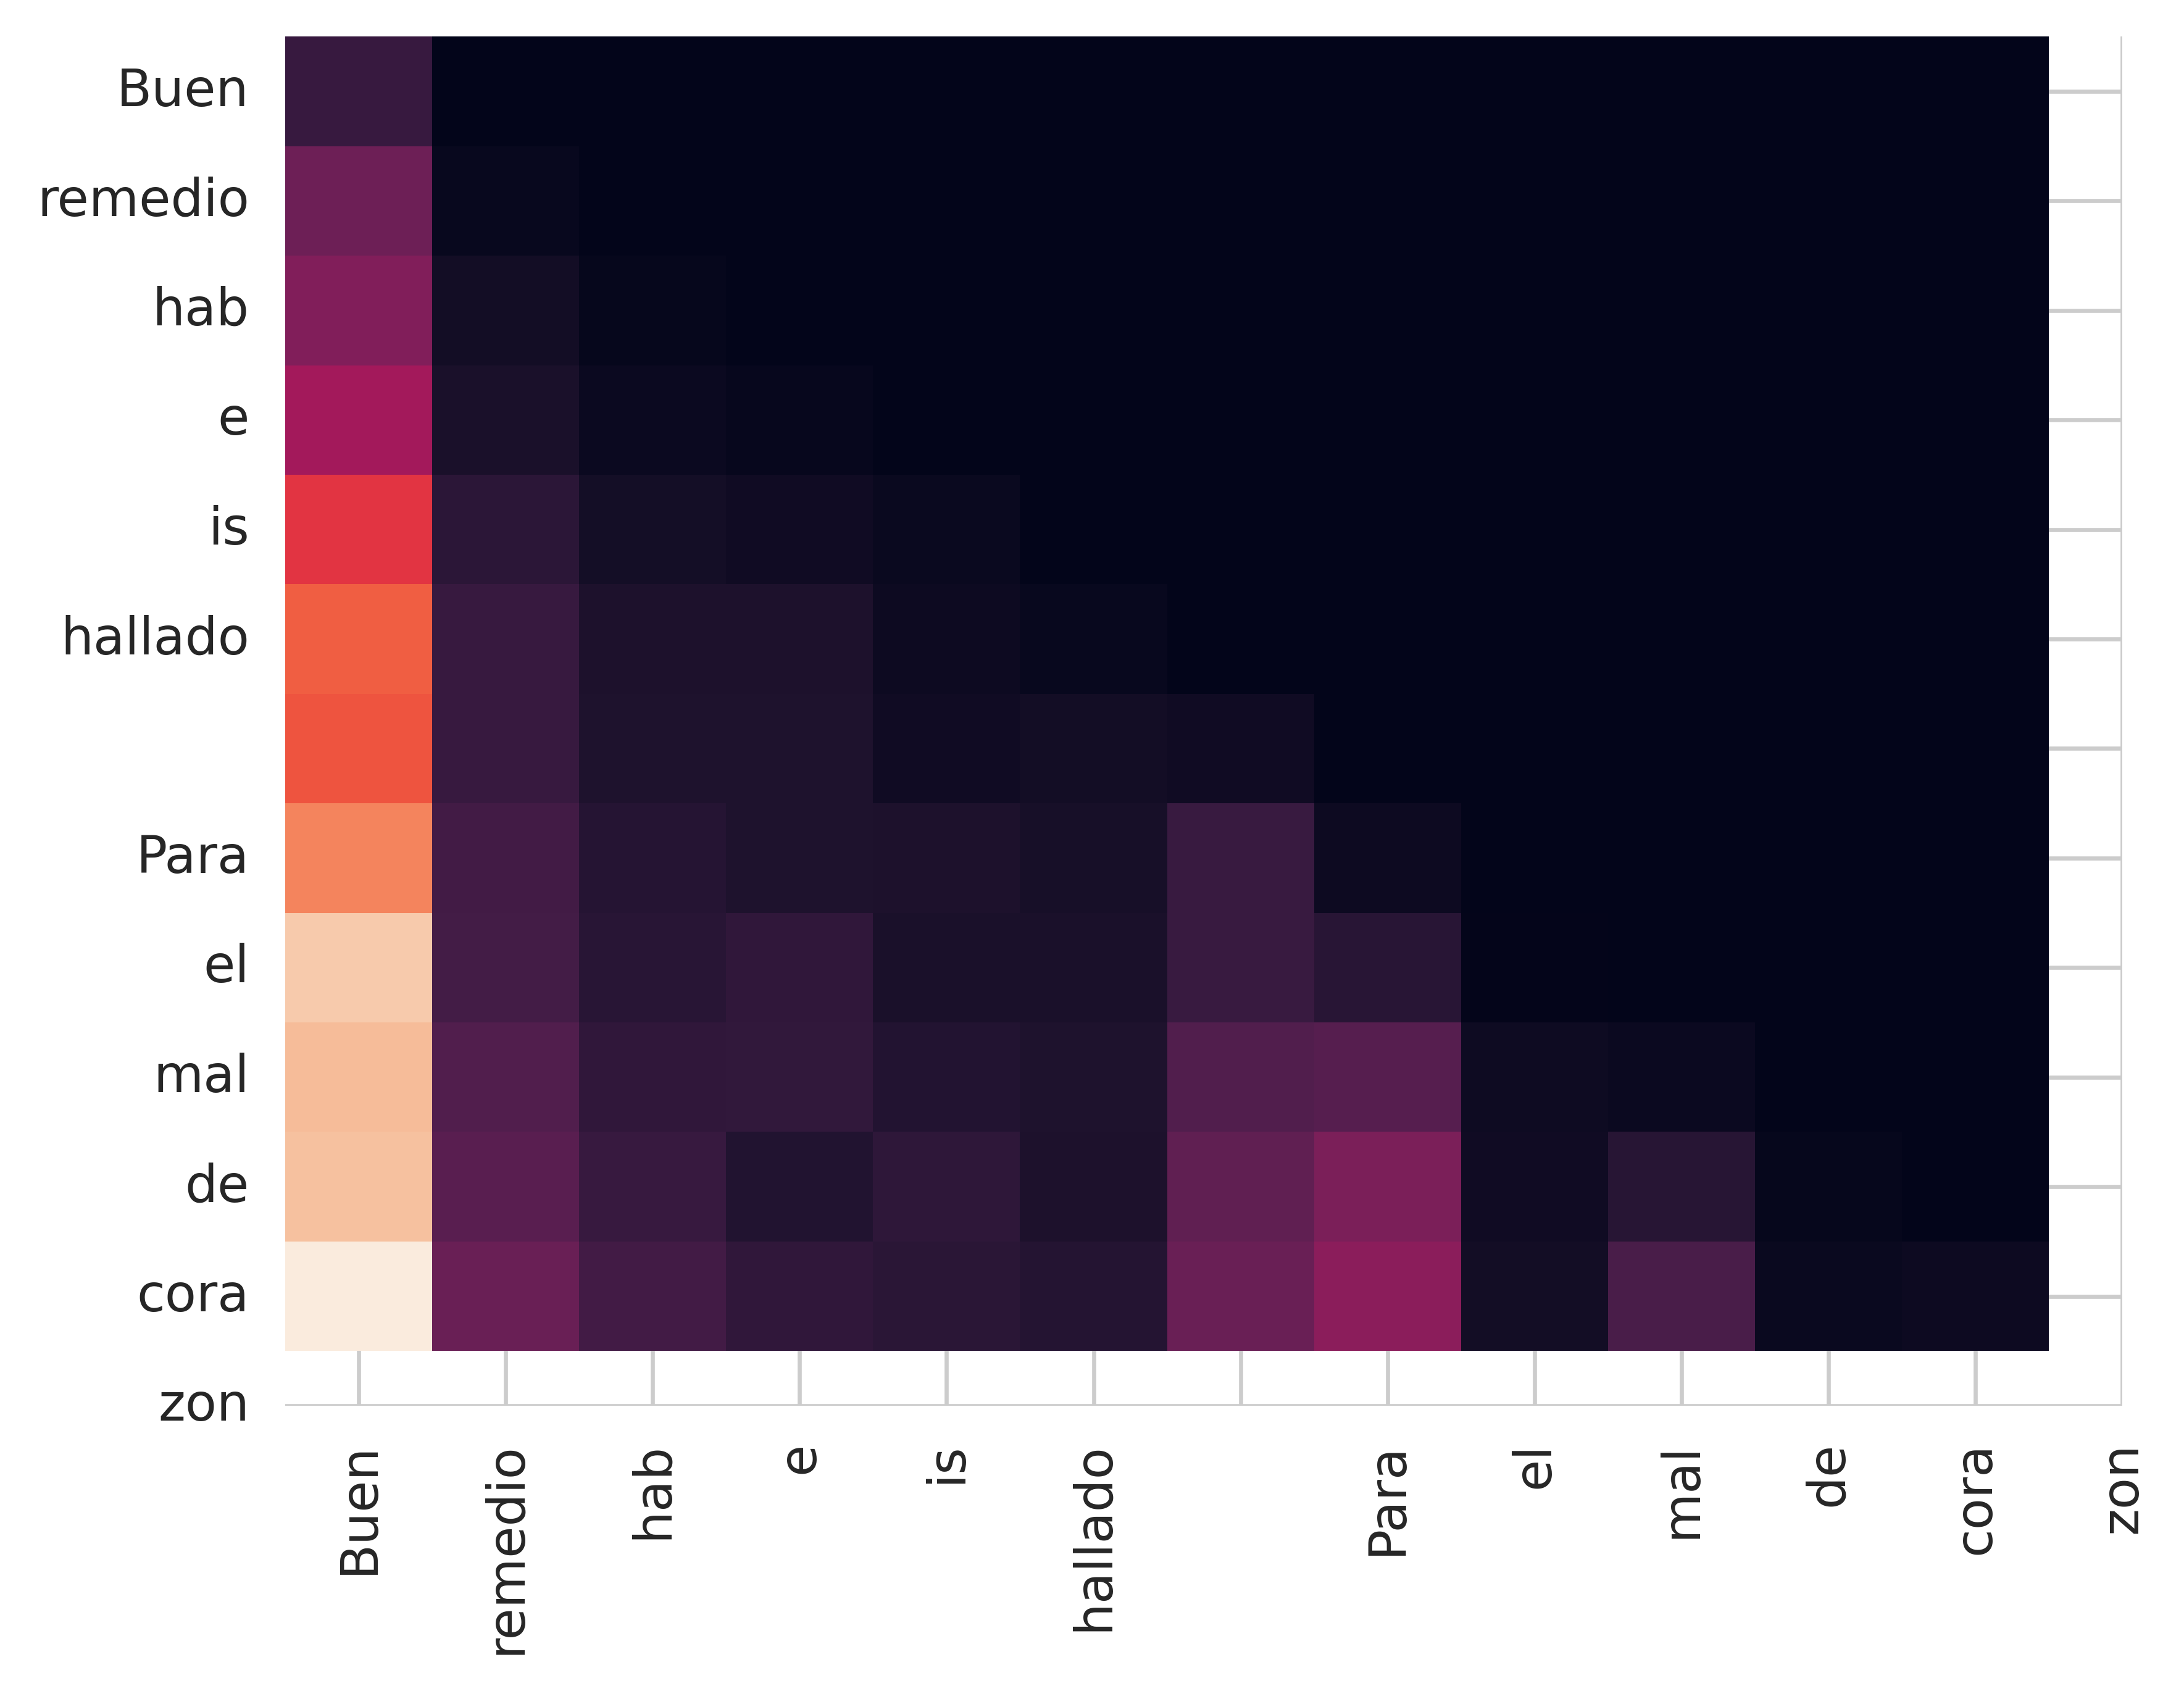
\includegraphics[width=\textwidth]{figures/chapter5/rollout_max.png}
        \caption{Despliegue de atención sobre la matriz de pesos de atención máxima}
    \end{subfigure}

    \caption{Mapa de calor representando el despliegue de atención sobre la secuencia  ``Buen remedio habeis hallado Para el mal de corazon'', en el modelo GPT-2 entrenado.}
    \label{fig:attention_rollout}
\end{figure}



